\documentclass{scrreprt}
\usepackage[utf8]{inputenc}
\usepackage{booktabs}
\usepackage{xcolor}
\usepackage{hyperref}
\usepackage{lmodern}
\usepackage[T1]{fontenc}
\usepackage{textcomp}
\usepackage{geometry}
\usepackage{float}
\usepackage{array}
\geometry{a4paper, margin=1in}
\usepackage{placeins} 
\usepackage{graphicx}
\usepackage{tabularx} %
\usepackage{longtable} %
\usepackage{array} %
\usepackage{ragged2e}
\usepackage{float} % 
\usepackage{multirow}


\newcounter{sprint}
\setcounter{sprint}{0}
\usepackage{longtable}
\usepackage{array}
\usepackage{multirow}

\hypersetup{
    pdftitle={Software Planning and UML},
    pdfauthor={Team 3 - PAO 2 2024},
    pdfsubject={TeX and LaTeX},
    pdfkeywords={TeX, LaTeX, graphics, images},
    colorlinks=true,
    linkcolor=blue,
    citecolor=black,
    filecolor=black,
    urlcolor=purple,
    linktoc=page
}
\def\myversion{1.0 }
\date{November 14, 2024}

\begin{document}

\begin{titlepage}
    \begin{flushright}
        \rule{16cm}{1.5pt} \\[1cm]
        {\Huge\bfseries SOFTWARE PLANNING\\ AND UML}\\[1cm]
        {\LARGE\bfseries for}\\[1cm]
        {\Huge\textbf{ESPOLTEL HIRING MANAGER}}\\[2cm]
        {\Large\textbf{Version \myversion}}\\[1.5cm]
        
        {\Large\textbf{Jeremy Rodrigo Poveda Gorotiza}\\
        \textbf{José David Ramos Rios}\\
        \textbf{Diego Fernando Flores Rengifo}\\
        \textbf{Ariana Valentina Palacios Saenz}\\
        \textbf{Alex Javier Vizuete Pereira}}\\[1.5cm]
        
        {\Large\textbf{Submitted to:} Francisco Ramirez}\\[1.5cm]
        {\Large\textbf{\today}}
    \end{flushright}
    \vfill
\end{titlepage}

\chapter*{Revision History}
\setcounter{page}{1}
\begin{center}
	\begin{tabular}{@{} l l p{6.5cm} l @{}}
		\toprule
		\textbf{Name}    & \textbf{Date}   & \textbf{Reason for Changes} & \textbf{Version} \\ 
		\midrule
		Team 3           & 2025-1-10      & Initial draft               & 1.0              \\
		\bottomrule
	\end{tabular}
\end{center}

\tableofcontents

\listoffigures
\listoftables



\chapter{Introduction}
\section{Summary}
This document presents a comprehensive framework for the design, planning, and execution of the ESPOLTEL HIRING MANAGER system. This product integrates a robust risk management strategy, a detailed project execution timeline, and a structured Sprint Backlog plan. Through the inclusion of Unified Modeling Language (UML) diagrams, we provide a thorough representation of both the static and behavioral logic of the system, ensuring that the architecture adheres to SOLID principles and eliminates implementation inefficiencies.

Our primary objective is to meticulously define the planning and breakdown of the system’s static structure, logical flow, behavioral processes, implementation strategies, and activity sequences. These components collectively support the realization of a user-centric, scalable, and maintainable product.

\section{Key features and Objetives}
The ESPOLTEL HIRING MANAGER product is designed to streamline and enhance the recruitment process, leveraging a combination of web and mobile modules for maximum efficiency. Key objectives include:

\begin{enumerate}
	\item \textbf{Risk Mitigation:} Developing a proactive risk management plan to address potential challenges in implementation and deployment.
	\item \textbf{Comprehensive Planning:} Structuring the project execution into manageable phases using Agile methodologies.
	\item \textbf{System Design:} Crafting static and behavioral UML diagrams to visualize the architecture, interactions, and workflows.
	\item \textbf{Adherence to SOLID Principles:} Ensuring maintainability and scalability by avoiding anti-patterns and promoting clean code practices.
\end{enumerate}

\chapter{Risk management, product and sprint backlogs and scheduling}
\section{Risk management}
In this section, we will identify, quantify, and classify the various risks that may arise during the software development process. Additionally, we will provide a detailed assessment of the likelihood of occurrence, the potential impact of each risk, and the corresponding protocols to be followed in the event they materialize.

%%
\begin{table}[h!]
	\centering \small
	\renewcommand{\arraystretch}{1.5} 
	\begin{tabular}{|p{10cm}|p{5cm}|} 
		\hline
		\textbf{Description} & \textbf{Probability Range} \\ \hline
		Not Probable: The event is highly unlikely to occur. & 0\% - 20\% \\ \hline
		Low Probability: The event is unlikely but possible. & 21\% - 40\% \\ \hline
		Moderate Probability: The event has an even chance of occurring. & 41\% - 60\% \\ \hline
		High Probability: The event is likely to occur. & 61\% - 80\% \\ \hline
		Very High Probability: The event is almost certain to occur. & 81\% - 100\% \\ \hline
	\end{tabular}
	\caption{Probability of Occurrence}
\end{table} \FloatBarrier
%%

%%

%%
\begin{table}[h!]
	\centering \small
	\renewcommand{\arraystretch}{1.5} 
	\begin{tabular}{|p{5cm}|p{10cm}|} 
		\hline
		\textbf{Impact Level} & \textbf{Description} \\ \hline
		Low Impact & Minimal effect on the project. No significant changes required. \\ \hline
		Moderate Impact & Some delays or adjustments needed but manageable within the team. \\ \hline
		High Impact & Significant disruptions, requiring immediate attention and resource allocation. \\ \hline
		Critical Impact & Severe consequences on project delivery, with major delays or failure possible. \\ \hline
	\end{tabular}
	\caption{Impact Levels}
\end{table} \FloatBarrier
%%
The following table outlines the identified risks associated with the project, including their probability of occurrence, potential impact, and the corresponding action protocol.
%%
\begin{table}[h!]
	\centering \small
	\renewcommand{\arraystretch}{1.5}
	\begin{tabular}{|p{.75cm}|p{4cm}|p{2.5cm}|p{2.5cm}|p{4.75cm}|} 
		\hline
		\textbf{Id} & \textbf{Name} & \textbf{Probability} & \textbf{Impact} & \textbf{Action Protocol} \\ \hline
		001 & Changes in requirements after development completion & High Probability & High Impact & Establish a communication protocol to clarify that no new requirements will be accepted after the design phase is finalized. \\ \hline
		002 & Discovery of implicit requirements not considered in the design & Very High Probability & High Impact & Accept and address the risk by updating the design and implementing the missing requirements. \\ \hline
		003 & Need for developer training & High Probability & High Impact & Provide immediate training on the required frameworks to minimize delays and ensure smooth development progress. \\ \hline
		004 & Difficulty understanding prior implementation, causing delays & Low Probability & Critical Impact & Reduce the probability by consulting previous implementers to gain insights into the system before development begins. \\ \hline
		005 & Schedule misalignment affecting task timelines & Not Probable & High Impact & Mitigate the risk by redistributing tasks and holding regular progress meetings to stay on track. \\ \hline
		006 & Performance drop due to prior monolithic architecture & Low Probability & High Impact & Accept the risk, inform the client, and propose alternative solutions to improve performance. \\ \hline
		007 & Database schema not designed for extensions & Low Probability & Moderate Impact & Accept the risk and adapt the existing schema to accommodate the new requirements. \\ \hline
		008 & Insufficient documentation provided by the client & High Probability & Critical Impact & Reduce probability by maintaining active communication with the client to obtain necessary documentation. \\ \hline
	\end{tabular}
	\caption{Risk Assessment and Action Protocols}
\end{table} \FloatBarrier
%%

\section{Product backlog}
\begin{longtable}{|p{0.8cm}|p{1.5cm}|p{2.5cm}|p{8cm}|p{2cm}|} \hline
	\textbf{ID} & \textbf{Priority} & \textbf{Dependencies} & \textbf{Item} & \textbf{Estimation (hours)} \\ \hline
	\endfirsthead
	\hline
	\textbf{ID} & \textbf{Priority} & \textbf{Dependencies} & \textbf{Item} & \textbf{Estimation (hours)} \\ \hline
	\endhead
	PB1 & 0 & None & Research Spring Boot  platform: Investigation of the architecture, modules, and functionalities of Spring Boot relevant to the project. Includes feasibility evaluation and the creation of a document with findings and recommendations. & 4 \\ \hline
	PB2 & 0 & None & Definition of the database schema: Design the database schema, including the definition of tables, relationships, and constraints. An Entity-Relationship diagram and the SQL script for database creation will be generated. & 8 \\ \hline
	
	%Register and loggin into the system
	
	PB3 & 1 & PB1, PB2 & \textbf{As} a user of ESPOLTEL Hiring Manager, \textbf{I want} to create my own account \textbf{so that} I can access all controls related to my role, ensuring my information and permissions are separate from other users. & 6 \\ \hline
	PB4 & 1 & PB3 & \textbf{As} a user of ESPOLTEL Hiring Manager, \textbf{I want} to verify my email address upon registration \textbf{so that} I can ensure secure access to the system and confirm my identity. & 8 \\ \hline
	PB5 & 2 & PB3 & \textbf{As} a user of ESPOLTEL Hiring Manager, \textbf{I want} to create my own account using the mobile app, \textbf{so that} I can access all controls corresponding to my role, and ensure that my information and permissions are separate from those of other users. & 6 \\ \hline
	PB6 & 1 & PB5 & \textbf{As} a user of ESPOLTEL Hiring Manager, \textbf{I want} to verify my email address when registering from my mobile device, \textbf{so that} I can ensure secure access to the system and confirm my identity. & 10 \\ \hline
	PB7 & 1 & PB3 & \textbf{As} a user of ESPOLTEL Hiring Manager, \textbf{I want} to log in securely using my credentials \textbf{so that} I can access features and project management tools. & 4\\ \hline
	PB8 & 1 & PB7 & \textbf{As} a user of ESPOLTEL Hiring Manager, \textbf{I want} to select my role (Aspirant, Project Manager, Project Director, or HR member) before logging in \textbf{so that} I am directed to the appropriate login process and access functionalities specific to my role. & 6 \\ \hline
	PB9 & 2 & PB7 & \textbf{As} a user of ESPOLTEL, \textbf{I want} to securely log in to the system using my credentials on my mobile device, \textbf{so that} I can access the appropriate functions and features according to my user role. & 5 \\ \hline
	PB10 & 2 & PB8 & \textbf{As} a user of ESPOLTEL, \textbf{I want} to be able to select my role (Aspirant, Project Manager, Project Director, or HR member) on my mobile device before logging in, \textbf{so that} I can be directed to the specific features and functionalities relevant to my role. &  6 \\ \hline
	PB11 & 3 & PB3 & \textbf{As} a user of ESPOLTEL Hiring Manager, \textbf{I want} to be able to recover my password through a secure and efficient process if I forget it, \textbf{so that} I can regain access to the system and continue with my responsibilities without delay. & 5 \\ \hline
	PB12 & 3 & PB5 & \textbf{As} a user of ESPOLTEL Hiring Manager, \textbf{I want} to be able to recover my password through a secure and efficient process by email from my mobile device if I forget it, \textbf{so that} I can regain access to the system and continue with my responsibilities without delay. & 6 \\ \hline
	
	%% Signer and FirmaEC
	PB13 & 2 & PB1,PB2 & \textbf{As} an aspirant or manager, \textbf{I want} to have access to contracts or confidential agreements pending my signature, \textbf{so that} I can review and sign them digitally within the web application. & 12 \\ \hline
	PB14 & 1 & P13 & \textbf{As} an aspirant, \textbf{I want} to upload my digital certificate to the platform \textbf{so that} I can sign documents such as contracts or confidentiality agreements for the projects I have applied to. & 5 \\ \hline
	PB15 & 1 & P13 & \textbf{As} a manager, \textbf{I want} to upload my digital certificate to the platform \textbf{so that} I can sign multiple documents such as contracts or confidentiality agreements for the projects I manage. & 5 \\ \hline
	PB16 & 1 & P14 & \textbf{As} an aspirant, \textbf{I want} to digitally sign my contract and confidentiality agreement \textbf{so that} I can complete the paperwork required for my hiring process. & 12 \\ \hline
	PB17 & 1 & P15 & \textbf{As} a manager, \textbf{I want} to digitally sign multiple documents, such as contracts or confidentiality agreements, simultaneously, \textbf{so that} I can save time and work more efficiently. & 12 \\ \hline
	PB18 & 3 & PB16 & \textbf{As} an aspirant, \textbf{I want} to view the contracts of the projects I have applied for and that are currently active, \textbf{so that} I have a clear view of the agreements I have signed. & 6 \\ \hline
	PB19 & 3 & PB18 & \textbf{As} an aspirant, \textbf{I want} to download the contracts of the projects I have applied for and that are currently active, \textbf{so that} I have a record of the agreements I have signed. & 4 \\ \hline
	PB20 & 3 & PB16 & \textbf{As} an aspirant, \textbf{I want} to view the contracts of the projects I have applied for and that are currently active on my smartphone, \textbf{so that} I have a clear view of the agreements I have signed. & 6 \\ \hline
	PB21 & 3 & PB20 & \textbf{As} an aspirant, \textbf{I want} to download the contracts of the projects I have applied for and that are currently active on my smartphone, \textbf{so that} I have a record of the agreements I have signed. & 4 \\ \hline
	PB22 & 1 & PB16 & \textbf{As} an HR member, \textbf{I want} to validate the digital signatures of aspirants \textbf{so that} I can ensure contracts and agreements are formalized. & 8 \\ \hline
	
	%% Project creation 
	PB23 & 2 & PB3 & \textbf{As} a project manager, \textbf{I want} to create a project by defining its name, description, start date, end date, and type, \textbf{so that} the project's objectives and timeline are clearly established. & 12 \\ \hline
	PB24 & 2 & PB23 & \textbf{As} a project manager, \textbf{I want} to define roles and profiles required for the project, including necessary skills and experience for each profile, \textbf{so that} aspirants can understand the requirements and apply to suitable positions. & 6 \\ \hline
	PB25 & 3 & PB24 & \textbf{As} a Director, \textbf{I want} to recommend an aspirant who has previously worked for ESPOLTEL for a role in a project, based on their past performance and experience, \textbf{so that} I have a worker I trust in my project. & 8 \\ \hline
	PB26 & 2 & PB24 & \textbf{As} an HR member, \textbf{I want} to validate the profiles created by project directors \textbf{so that} I can edit, approve, the profiles and positions defined for a project, ensuring they align with the company's standards and requirements. & 12 \\ \hline
	PB27 & 2 & PB23 & \textbf{As} a project manager or director at ESPOLTEL, \textbf{I want} to monitor on my smartphone the projects under my supervision, \textbf{so that} I can maintain better control and make informed decisions. & 8 \\ \hline
	PB28 & 2 & PB23 & \textbf{As} a Director or Manager, \textbf{I want} to view the resources and budget assigned to my project, \textbf{so that} I can track project expenses and resource utilization. & 10 \\ \hline
	%%

	%Apply for a project aspirant
	PB29 & 1 & PB8 & \textbf{As} an aspirant, \textbf{I want} to apply for a position in a project of interest where I meet the required profile \textbf{so that} I can obtain the desired position. & 10 \\ \hline
	PB30& 2 & PB29 & \textbf{As} an aspirant, \textbf{I want} to cancel my postulation for a specific role or hiring profile, \textbf{so that} I can withdraw from a recruitment process if my circumstances change. & 8 \\ \hline
	
	%% Interviews
	PB31& 2 & PB8, PB29& \textbf{As} an HR member, \textbf{I want} to schedule interviews with aspirants, specifying the date, time, and interviewer, \textbf{so that} the selection process can be efficiently conducted. & 10 \\ \hline
	PB32 & 2 & PB31 & \textbf{As} a HR member, \textbf{I want} to record interview results and observations, including scores and comments, \textbf{so that} there is a formal record of each aspirant's evaluation. & 8 \\ \hline
	PB33 & 2 & PB24, PB29 & \textbf{As} an HR member, \textbf{I want} to verify the requirements based on the information of an aspirant, \textbf{so that} I can ensure they meet the necessary qualifications for a project. & 8 \\ \hline
	PB34& 3 & PB32 & \textbf{As} an HR member, \textbf{I want} to add private comments in aspirants' postulations \textbf{so that} I can keep a record of observations and notes during the selection process. & 4 \\ \hline
	PB35 & 2 & PB32, PB33, PB34 & \textbf{As} an HR member, \textbf{I want} to select the best aspirants based on interview results and fulfilled requirements, \textbf{so that} I can identify the most suitable candidates for each role. & 10 \\ \hline
	
	%%Generate format documents
	PB36 & 2 & PB8 & \textbf{As} an HR member, \textbf{I want} to create and manage forms for pre-hiring and hiring processes, defining mandatory fields and document uploads, \textbf{so that} aspirants can provide the necessary information. & 15 \\ \hline
	PB37 & 2 & PB8 & \textbf{As} an HR member, \textbf{I want} to upload templates for contracts and agreements, \textbf{so that} appropriate templates are available for generating personalized documents for aspirants. & 12 \\ \hline
	PB38 & 2 & PB29, PB36 & \textbf{As} an aspirant, \textbf{I want} to upload my personal documents (such as CV, ID, certificates, etc.) and relevant information \textbf{by completing forms defined by HR,} \textbf{so that} I can fulfill postulation requirements. & 8 \\ \hline
	PB39 & 2 & PB37 & \textbf{As} an HR member, \textbf{I want} to generate contracts and agreements from templates, \textbf{so that} I can save time in creating personalized documents. & 12 \\ \hline
	
	%%Search and filter
	PB40 & 2 & PB32, PB33, PB34  & \textbf{As} an HR member, \textbf{I want} to view aspirants by specific skills and experience, \textbf{so that} I can make it easier to select candidates who meet the project requirements. & 4 \\ \hline
	PB41 & 2 & PB8 & \textbf{As} a Director, HR Member, or Manager, \textbf{I want} to view the hires or personnel associated with a project, \textbf{so that} I have an overview of the team composition and recruitment progress. & 10 \\ \hline
	PB42 & 2 & None & \textbf{As} a user of ESPOLTEL Hiring Manager, \textbf{I want} to be able to search and filter information across the platform, including projects, aspirants, roles, documents, and other relevant data, \textbf{so that} I can quickly find and focus on the data I need. & 8 \\ \hline
	
	%Notifications 
	PB43 & 1 & PB10 & \textbf{As} a user of the ESPOLTEL Hiring Manager mobile app, \textbf{I need} to receive notifications for any important events in the recruitment process, \textbf{so that} I can stay informed and respond promptly. & 12 \\ \hline
	PB44 & 2 & PB8 & \textbf{As} an aspirant, \textbf{I want} to monitor on my smartphone the projects I have applied for, \textbf{so that} I can stay updated on their progress and better manage my involvement. & 10 \\ \hline
	PB45 & 2 & PB31 & \textbf{As} an aspirant, \textbf{I want} to receive notifications about my scheduled interviews, including reminders and updates, \textbf{so that} I can be prepared and attend interviews on time. & 8 \\ \hline
	
	%% Testing
	PB46 & 4 & PB45 & Testing and deployment& 24\\ \hline
	\caption{Product Backlog of ESPOLTEL Hiring Manager}
\end{longtable}

\section{Sprint backlog}

\begin{longtable}{|p{1.5cm}|p{5.5cm}|p{4.5cm}|p{3cm}|} \hline
	\textbf{Product Backlog Item} & \textbf{User Story} & \textbf{Tasks} & \textbf{Assigned To} \\ \hline
	\endfirsthead
	\hline
	\textbf{Product Backlog Item} & \textbf{User Story} & \textbf{Tasks} & \textbf{Assigned To} \\ \hline
	\endhead
	
	PB1 & Research Spring Boot platform (4 hours) & 

	-Research architecture, modules, and functionalities of Spring Boot. - 3 hours\newline
	-Feasibility evaluation of this framework. - 1 hour 
	&
	- Jeremy Poveda, Diego Flores, Ariana Palacios\newline
	- Alex Vizuete, Jose Ramos
	\\ \hline
	
	PB2 & Definition of the database schema (8 hours) & 
	-Design the database schema (tables, relationships, and constraints). - 4 hours\newline
	-Generate Entity-Relationship diagram and SQL script. - 4 hours
	&
	- Diego Flores, Ariana Palacios\newline
	- Jeremy Poveda, Alex Vizuete
	\\ \hline
	PB3 & \textbf{As} a user of ESPOLTEL Hiring Manager, \textbf{I want} to create my own account \textbf{so that} I can access all controls related to my role, ensuring my information and permissions are separate from other users. (6 hours) & 
	- Design UI for user registration (web). - 2 hours \newline
	- Implement backend logic for user registration and role management. - 3 hours \newline
	- Database integration for user accounts. - 1 hour 
	&
	- Jeremy Poveda \newline
	- Jose Ramos \newline
	- Ariana Palacios
	\\ \hline
	
	PB4 & \textbf{As} a user of ESPOLTEL Hiring Manager, \textbf{I want} to verify my email address upon registration \textbf{so that} I can ensure secure access to the system and confirm my identity. (8 hours) & 
	- Implement email sending functionality (e.g., using Spring Mail). - 3 hours \newline
	- Create email verification endpoint. - 3 hours \newline
	- Integrate email verification with registration flow. - 2 hours
	&
	- Alex Vizuete \newline
	- Diego Flores \newline
	- Jeremy Poveda
	\\ \hline
	
	PB5 & \textbf{As} a user of ESPOLTEL Hiring Manager, \textbf{I want} to create my own account using the mobile app, \textbf{so that} I can access all controls corresponding to my role, and ensure that my information and permissions are separate from those of other users. (6 hours) & 
	- Design UI for user registration (mobile). - 2 hours \newline
	- Implement backend logic for user registration and role management (mobile). - 3 hours \newline
	- Database integration for user accounts (mobile). - 1 hour
	&
	- Diego Flores \newline
	- Jose Ramos \newline
	- Ariana Palacios
	\\ \hline
	
	PB6 & \textbf{As} a user of ESPOLTEL Hiring Manager, \textbf{I want} to verify my email address when registering from my mobile device, \textbf{so that} I can ensure secure access to the system and confirm my identity. (10 hours) & 
	- Adapt email sending functionality for mobile. - 3 hours \newline
	- Create email verification endpoint (mobile). - 4 hours \newline
	- Integrate email verification with mobile registration flow. - 3 hours
	&
	- Alex Vizuete \newline
	- Jeremy Poveda \newline
	- Jose Ramos
	\\ \hline
	
	PB7 & \textbf{As} a user of ESPOLTEL Hiring Manager, \textbf{I want} to log in securely using my credentials \textbf{so that} I can access features and project management tools. (4 hours)& 
- Design UI for user login (web). - 1 hour \newline
- Implement backend logic for authentication. - 2 hours \newline
- Implement session management. - 1 hour
&
- Jose Ramos \newline
- Ariana Palacios \newline
- Alex Vizuete
\\ \hline

PB8 & \textbf{As} a user of ESPOLTEL Hiring Manager, \textbf{I want} to select my role (Aspirant, Project Manager, Project Director, or HR member) before logging in \textbf{so that} I am directed to the appropriate login process and access functionalities specific to my role. (6 hours) & 
- Design UI for role selection. - 3 hours \newline
- Implement role-based access control logic. - 3 hours
&
- Diego Flores \newline
- Jeremy Poveda
\\ \hline
PB9 & \textbf{As} a user of ESPOLTEL, \textbf{I want} to securely log in to the system using my credentials on my mobile device, \textbf{so that} I can access the appropriate functions and features according to my user role. (5 hours) &
- Design UI for user login (mobile). - 2 hours \newline
- Implement backend logic for authentication (mobile). - 2 hours \newline
- Implement session management (mobile). - 1 hour
&
- Jeremy Poveda \newline
- Ariana Palacios \newline
- Alex Vizuete
\\ \hline

PB10 & \textbf{As} a user of ESPOLTEL, \textbf{I want} to be able to select my role (Aspirant, Project Manager, Project Director, or HR member) on my mobile device before logging in, \textbf{so that} I can be directed to the specific features and functionalities relevant to my role. (6 hours) & 
- Design UI for role selection (mobile). - 3 hours \newline
- Implement role-based access control logic (mobile). - 3 hours
&
- Diego Flores \newline
- Jose Ramos
\\ \hline

PB11 & \textbf{As} a user of ESPOLTEL Hiring Manager, \textbf{I want} to be able to recover my password through a secure and efficient process if I forget it, \textbf{so that} I can regain access to the system and continue with my responsibilities without delay. (5 hours) & 
- Design UI for password recovery. - 2 hours \newline
- Implement backend logic for password recovery. - 3 hours
&
- Jose Ramos \newline
- Ariana Palacios
\\ \hline
PB12 & \textbf{As} a user of ESPOLTEL Hiring Manager, \textbf{I want} to be able to recover my password through a secure and efficient process by email from my mobile device if I forget it, \textbf{so that} I can regain access to the system and continue with my responsibilities without delay. (6 hours) &
- Design UI for password recovery (mobile). - 2 hours \newline
- Implement backend logic for password recovery, including email sending (mobile). - 3 hours\newline
- Integrate password recovery with mobile login flow. - 1 hour
&
- Diego Flores \newline
- Ariana Palacios \newline
- Alex Vizuete
\\ \hline

\caption{Sprint 1 of ESPOLTEL Hiring Manager}
\end{longtable}

%%Sprint 2
\begin{longtable}{|p{1.5cm}|p{5.5cm}|p{4.5cm}|p{3cm}|} \hline
	\textbf{Product Backlog Item} & \textbf{User Story} & \textbf{Tasks} & \textbf{Assigned To} \\ \hline
	\endfirsthead
	\hline
	\textbf{Product Backlog Item} & \textbf{User Story} & \textbf{Tasks} & \textbf{Assigned To} \\ \hline
	\endhead
	
	PB13 & \textbf{As} an aspirant or manager, \textbf{I want} to have access to contracts or confidential agreements pending my signature, \textbf{so that} I can review and sign them digitally within the web application. (12) &
	
	Design UI for contract/agreement viewing. - 4 hours \newline
	Implement backend logic for fetching pending documents. - 4 hours \newline
	Integrate digital signature service/library. - 4 hours &
	Jeremy Poveda \newline
	Jose Ramos \newline
	Alex Vizuete \\ \hline
	
	PB14 & \textbf{As} an aspirant, \textbf{I want} to upload my digital certificate to the platform \textbf{so that} I can sign documents such as contracts or confidentiality agreements for the projects I have applied to. (5) &
	
	Design UI for digital certificate upload. - 2 hours \newline
	Implement backend logic for certificate storage and validation. - 3 hours &
	Diego Flores \newline
	Ariana Palacios \\ \hline
	
	PB15 & \textbf{As} a manager, \textbf{I want} to upload my digital certificate to the platform \textbf{so that} I can sign multiple documents such as contracts or confidentiality agreements for the projects I manage. (5) &
	
	Design UI for digital certificate upload (Manager). - 2 hours \newline
	Implement backend logic for certificate storage and validation (Manager). - 3 hours &
	Jeremy Poveda \newline
	Alex Vizuete \\ \hline
	
	PB16 & \textbf{As} an aspirant, \textbf{I want} to digitally sign my contract and confidentiality agreement \textbf{so that} I can complete the paperwork required for my hiring process. (12) & 
	
	Integrate digital signature functionality for aspirants. - 6 hours \newline
	Design UI for signing contracts and agreements. - 3 hours \newline
	Update database to store signature data and status. - 3 hours & 
	Diego Flores \newline
	Jeremy Poveda \\ \hline 
	
	
	PB17 & \textbf{As} a manager, \textbf{I want} to digitally sign multiple documents, such as contracts or confidentiality agreements, simultaneously, \textbf{so that} I can save time and work more efficiently. (12) &
	
	Implement bulk/batch digital signature functionality. - 8 hours \newline
	Design UI for bulk signing. - 2 hours \newline
	Update backend logic to handle multiple signatures. - 2 hours &
	Diego Flores \newline
	Ariana Palacios \newline
	Jeremy Poveda \\ \hline
	
	PB18 & \textbf{As} an aspirant, \textbf{I want} to view the contracts of the projects I have applied for and that are currently active, \textbf{so that} I have a clear view of the agreements I have signed. (6) &
	Design UI for contract viewing (aspirant). - 3 hours \newline
	Implement backend logic for fetching and displaying active contracts. - 3 hours &
	Alex Vizuete \newline
	Jose Ramos \\ \hline
	
	PB19 & \textbf{As} an aspirant, \textbf{I want} to download the contracts of the projects I have applied for and that are currently active, \textbf{so that} I have a record of the agreements I have signed. (4) &
	Implement contract download functionality. - 2 hours \newline
	Integrate with secure document storage. - 2 hours &
	Alex Vizuete \newline
	Jose Ramos \\ \hline
	
	PB20 & \textbf{As} an aspirant, \textbf{I want} to view the contracts of the projects I have applied for and that are currently active on my smartphone, \textbf{so that} I have a clear view of the agreements I have signed. (6) &
	Design mobile UI for contract viewing. - 3 hours \newline
	Adapt backend logic for mobile contract fetching. - 3 hours &
	Diego Flores \newline
	Ariana Palacios \\ \hline
	
	PB21 & \textbf{As} an aspirant, \textbf{I want} to download the contracts of the projects I have applied for and that are currently active on my smartphone, \textbf{so that} I have a record of the agreements I have signed. (4) &
	Implement mobile contract download functionality. - 2 hours \newline
	Integrate with mobile secure storage. - 2 hours &
	Diego Flores \newline
	Jose Ramos \\ \hline
	
	
	PB22 & \textbf{As} an HR member, \textbf{I want} to validate the digital signatures of aspirants \textbf{so that} I can ensure contracts and agreements are formalized. (8) &
	
	Implement backend logic for signature validation. - 5 hours \newline
	Design UI for displaying signature validation status. - 3 hours &
	Ariana Palacios \newline
	Jose Ramos\\ \hline
	
	PB23 & \textbf{As} a project manager, \textbf{I want} to create a project by defining its name, description, start date, end date, and type, \textbf{so that} the project's objectives and timeline are clearly established. (12) &
	
	Design UI for project creation form. - 4 hours \newline
	Implement backend logic for project creation and data validation. - 5 hours \newline
	Database integration for project data. - 3 hours &
	Jose Ramos \newline
	Ariana Palacios \newline
	Diego Flores \\ \hline
	
	PB24 & \textbf{As} a project manager, \textbf{I want} to define roles and profiles required for the project, including necessary skills and experience for each profile, \textbf{so that} aspirants can understand the requirements and apply to suitable positions. (6) &
	
	Design UI for role/profile definition. - 3 hours \newline
	Implement backend logic for storing role/profile data. - 3 hours &
	Jose Ramos \newline
	Alex Vizuete \\ \hline
	
	PB25 & \textbf{As} a Director, \textbf{I want} to recommend an aspirant who has previously worked for ESPOLTEL for a role in a project, based on their past performance and experience, \textbf{so that} I have a worker I trust in my project. (8) &
	Design UI for aspirant recommendation. - 3 hours \newline
	Implement backend logic for recommendation processing, including fetching past performance data. - 5 hours &
	Jeremy Poveda \newline
	Alex Vizuete \\ \hline
	
	PB26 & \textbf{As} an HR member, \textbf{I want} to validate the profiles created by project directors \textbf{so that} I can edit, approve, the profiles and positions defined for a project, ensuring they align with the company's standards and requirements. (12) &
	
	Design UI for profile review and approval. - 4 hours \newline
	Implement backend logic for profile validation workflow. - 5 hours \newline
	Database integration for profile status. - 3 hours &
	Ariana Palacios \newline
	Diego Flores \newline
	Jeremy Poveda \\ \hline
	
	PB27 & \textbf{As} a project manager or director at ESPOLTEL, \textbf{I want} to monitor on my smartphone the projects under my supervision, \textbf{so that} I can maintain better control and make informed decisions. (8) &
	Design mobile UI for project monitoring. - 4 hours \newline
	Implement mobile backend logic for retrieving project data. - 4 hours &
	Diego Flores \newline
	Jose Ramos \\ \hline
	
	PB28 & \textbf{As} a Director or Manager, \textbf{I want} to view the resources and budget assigned to my project, \textbf{so that} I can track project expenses and resource utilization. (10) &
	Design UI for resource and budget viewing. - 4 hours \newline
	Implement backend logic for retrieving resource and budget data. - 6 hours &
	Ariana Palacios \newline
	Alex Vizuete \\ \hline
	
	\caption{Sprint 2 of ESPOLTEL Hiring Manager}
\end{longtable}

%% Sprint 3
\begin{longtable}{|p{1.5cm}|p{5.5cm}|p{4.5cm}|p{3cm}|} \hline
	\textbf{Product Backlog Item} & \textbf{User Story} & \textbf{Tasks} & \textbf{Assigned To} \\ \hline
	\endfirsthead
	\hline
	\textbf{Product Backlog Item} & \textbf{User Story} & \textbf{Tasks} & \textbf{Assigned To} \\ \hline
	\endhead
	
	
	PB29 & \textbf{As} an aspirant, \textbf{I want} to apply for a position in a project of interest where I meet the required profile \textbf{so that} I can obtain the desired position. (10) & 
	Design UI for project/position application. - 4 hours \newline
	Implement backend logic for application processing. - 6 hours & 
	Alex Vizuete \newline 
	Jose Ramos \\ \hline
	
	PB30 & \textbf{As} an aspirant, \textbf{I want} to cancel my postulation for a specific role or hiring profile, \textbf{so that} I can withdraw from a recruitment process if my circumstances change. (8) & 
	Design UI for postulation cancellation. - 3 hours \newline
	Implement backend logic for postulation cancellation. - 5 hours & 
	Jeremy Poveda \newline 
	Diego Flores \\ \hline
	
	
	% Interviews
	PB31 & \textbf{As} an HR member, \textbf{I want} to schedule interviews with aspirants, specifying the date, time, and interviewer, \textbf{so that} the selection process can be efficiently conducted. (10) &
	Design UI for interview scheduling. - 4 hours \newline
	Implement backend logic for interview scheduling and notifications. - 6 hours &
	Diego Flores \newline
	Ariana Palacios \\ \hline
	
	PB32 & \textbf{As} an HR member, \textbf{I want} to record interview results and observations, including scores and comments, \textbf{so that} there is a formal record of each aspirant's evaluation. (8) &
	Design UI for recording interview results. - 3 hours \newline
	Implement backend logic for storing interview data. - 5 hours &
	Jeremy Poveda \newline
	Diego Flores \\ \hline
	
	PB33 & \textbf{As} an HR member, \textbf{I want} to verify the requirements based on the information of an aspirant, \textbf{so that} I can ensure they meet the necessary qualifications for a project. (8) &
	Design UI for requirement verification. - 3 hours \newline
	Implement backend logic for requirement checking. - 5 hours &
	Jose Ramos \newline
	Ariana Palacios \\ \hline
	
	PB34 & \textbf{As} an HR member, \textbf{I want} to add private comments in aspirants' postulations \textbf{so that} I can keep a record of observations and notes during the selection process. (4) &
	Design UI for adding private comments. - 2 hours \newline
	Implement backend logic for storing private comments. - 2 hours &
	Alex Vizuete \newline
	Jeremy Poveda \\ \hline
	
	PB35 & \textbf{As} an HR member, \textbf{I want} to select the best aspirants based on interview results and fulfilled requirements, \textbf{so that} I can identify the most suitable candidates for each role. (10) &
	Design UI for aspirant selection. - 4 hours \newline
	Implement backend logic for selection processing. - 6 hours &
	Diego Flores \newline
	Jose Ramos \\ \hline
	
	% Generate format documents
	PB36 & \textbf{As} an HR member, \textbf{I want} to create and manage forms for pre-hiring and hiring processes, defining mandatory fields and document uploads, \textbf{so that} aspirants can provide the necessary information. (15) &
	Design UI for form creation and management. - 5 hours \newline
	Implement backend logic for form data storage and retrieval. - 7 hours \newline
	Integrate document upload functionality. - 3 hours &
	Jose Ramos \newline
	Alex Vizuete \newline
	Ariana Palacios \\ \hline
	
	PB37 & \textbf{As} an HR member, \textbf{I want} to upload templates for contracts and agreements, \textbf{so that} appropriate templates are available for generating personalized documents for aspirants. (12) &
	Design UI for template upload and management. - 4 hours \newline
	Implement backend logic for template storage and retrieval. - 5 hours \newline
	Implement template versioning. - 3 hours &
	Jeremy Poveda \newline
	Jose Ramos \newline
	Alex Vizuete \\ \hline
	
	PB38 & \textbf{As} an aspirant, \textbf{I want} to upload my personal documents (such as CV, ID, certificates, etc.) and relevant information \textbf{by completing forms defined by HR,} \textbf{so that} I can fulfill postulation requirements. (8) &
	Implement document upload and form submission functionality. - 5 hours \newline
	Update UI to integrate with forms defined by HR. - 3 hours &
	Ariana Palacios \newline
	Alex Vizuete \\ \hline
	
	PB39 & \textbf{As} an HR member, \textbf{I want} to generate contracts and agreements from templates, \textbf{so that} I can save time in creating personalized documents. (12) &
	Implement backend logic for document generation from templates. - 8 hours \newline
	Design UI for document generation. - 4 hours &
	Ariana Palacios \newline
	Diego Flores \newline
	Jeremy Poveda \\ \hline
	
	\caption{Sprint 3 of ESPOLTEL Hiring Manager}
\end{longtable}

\begin{longtable}{|p{1.5cm}|p{5.5cm}|p{4.5cm}|p{3cm}|} \hline
	\textbf{Product Backlog Item} & \textbf{User Story} & \textbf{Tasks} & \textbf{Assigned To} \\ \hline
	\endfirsthead
	\hline
	\textbf{Product Backlog Item} & \textbf{User Story} & \textbf{Tasks} & \textbf{Assigned To} \\ \hline
	\endhead
	
	 % Search and filter
	PB40 & \textbf{As} an HR member, \textbf{I want} to view aspirants by specific skills and experience, \textbf{so that} I can make it easier to select candidates who meet the project requirements. (4) &
	Enhance search/filter functionality for aspirants. - 4 hours &
	Jeremy Poveda \newline
	Diego Flores \\ \hline
	
	PB41 & \textbf{As} a Director, HR Member, or Manager, \textbf{I want} to view the hires or personnel associated with a project, \textbf{so that} I have an overview of the team composition and recruitment progress. (10) &
	Design UI for viewing project personnel. - 4 hours \newline
	Implement backend logic for retrieving project personnel data. - 6 hours &
	Jose Ramos \newline
	Alex Vizuete \\ \hline
	
	PB42 & \textbf{As} a user of ESPOLTEL Hiring Manager, \textbf{I want} to be able to search and filter information across the platform, including projects, aspirants, roles, documents, and other relevant data, \textbf{so that} I can quickly find and focus on the data I need. (8) &
	Design UI for search and filter functionality. - 3 hours \newline
	Implement backend logic for search and filtering. - 5 hours &
	Alex Vizuete \newline
	Jeremy Poveda \\ \hline
	
	% Notifications
	PB43 & \textbf{As} a user of the ESPOLTEL Hiring Manager mobile app, \textbf{I need} to receive notifications for any important events in the recruitment process, \textbf{so that} I can stay informed and respond promptly. (12) &
	Set up push notification service (e.g., Firebase Cloud Messaging). - 4 hours \newline
	Implement backend logic to trigger notifications. - 4 hours \newline
	Integrate notifications with mobile app. - 4 hours &
	Diego Flores \newline
	Jose Ramos \newline
	Ariana Palacios \\ \hline
	
	PB44 & \textbf{As} an aspirant, \textbf{I want} to monitor on my smartphone the projects I have applied for, \textbf{so that} I can stay updated on their progress and better manage my involvement. (10) &
	Design mobile UI for application monitoring. - 4 hours \newline
	Implement mobile backend logic for retrieving application status. - 6 hours &
	Jose Ramos \newline
	Ariana Palacios \\ \hline
	
	PB45 & \textbf{As} an aspirant, \textbf{I want} to receive notifications about my scheduled interviews, including reminders and updates, \textbf{so that} I can be prepared and attend interviews on time. (8) &
	Implement notification logic for interview scheduling. - 5 hours \newline
	Integrate with calendar/reminder system if needed. - 3 hours &
	Jeremy Poveda \newline
	Alex Vizuete \\ \hline
	
	% Testing
	PB46 & Testing and deployment (24) &
	Functional testing. - 8 hours \newline
	Integration testing. - 8 hours \newline
	Performance testing. - 4 hours \newline
	Deployment to staging/production. - 4 hours &
	All team members \\ \hline
	
	\caption{Sprint 4 of ESPOLTEL Hiring Manager}
\end{longtable}

\section{Scheduling}
\begin{table}[h]
	\centering
	\begin{tabular}{|p{.5cm}|p{3cm}|p{1cm}|p{3cm}|p{1cm}|p{1.5cm}|p{1.5cm}|p{1.5cm}|}
		\hline
		\textbf{ID} & \textbf{Description} & \textbf{Dep} & \textbf{Product Backlog Items} & \textbf{Hours} & \textbf{Earliest Start Time}& \textbf{Lastest Finish Time}& \textbf{Float}\\ \hline
		A &  System Foundation & None & PB1, PB2 & 12 & 0 & 12 & 0 \\ \hline
		B & User Management & A & PB3, PB4, PB5, PB6, PB7, PB8, PB9, PB10, PB11, PB12 & 62 & 12 & 74 & 0\\ \hline
		C & Digital Signature & B &  PB13, PB14, PB15, PB16, PB17, PB18, PB19, PB20, PB21, PB22 & 74  & 74  & 249 & 101 \\ \hline
		D & Project Creation & B & PB23, PB24, PB25, PB26, PB27, PB28 & 56 & 74 & 130 &  0 \\ \hline
		E & Aspirant Postulation & D & PB29, PB30 & 18 & 130 & 148 & 0 \\ \hline
	    F & Interviews & D, E & PB31, PB32, PB33, PB34, PB35 & 40 & 148 & 227 & 39 \\ \hline
		G & Document Generation & E & PB36, PB37, PB38, PB39 & 47 & 148 & 195 & 0 \\ \hline
		H & Search and Filtering &  E, F  & PB40, PB41, PB42 & 22 & 188 & 249 & 39 \\ \hline
		I & Notifications & G  & PB43, PB44, PB45 & 30 & 195 & 225 & 0 \\ \hline
		J & Testing and Deployment & I & PB46 & 24 & 225 & 249 & 0 \\ \hline 
	\end{tabular}
	\caption{Activity Arrow table for Macro-activities ESPOLTEL Hiring Manager}
	\label{Activities}
\end{table}

\begin{figure}[h!]
	\centering
	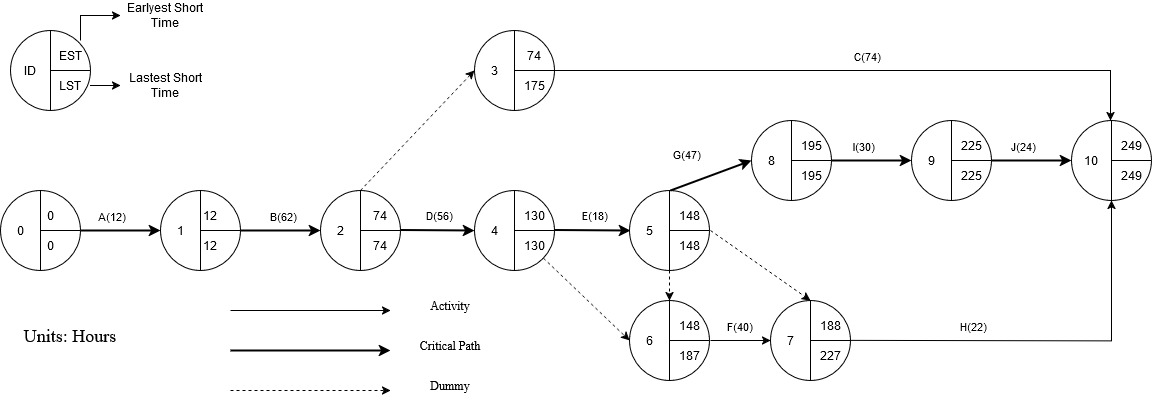
\includegraphics[width=17cm]{ActivityArrowDiagram.png} 
	\caption{Activity Arrow Diagram of ESPOLTEL HIRING MANAGER}
	\label{fig:ActivityArrowDiagram}
\end{figure}

\chapter{Static UML}
\section{Use Case - Web Module}
\section{Use Case - Mobile Module}



\chapter{Behavior UML}

    
\chapter{Individual Contributions}
\vspace{2cm}

\begin{table}[h!]
    \centering \small
    \renewcommand{\arraystretch}{1.5} % Aumenta el espacio entre filas
    \begin{tabular}{|p{5cm}|p{10cm}|} % Ajusta el ancho de las columnas
    \hline
    \textbf{Student's Names} & \textbf{Contributions} \\ \hline
    Jeremy Rodrigo Poveda Gorotiza & Project Scope, Introduction, User Stories, Creation of GitHub Repository, prototype: web application for director and managers \\ \hline
    Diego Fernando Flores Rengifo & Non functional requirements both Web and Mobile Application, prototype in figma: Authentification module and aspirants Platform  \\ \hline
    José David Ramos Rios & Product Overview, Product Features, Module Featuring: Mobile App, First Preview of Module Featuring: Web Application, and prototype in figma of Mobile App \\ \hline
    Ariana Valentina Palacios Saenz & Revision, User Stories, and prototyping flows and module integration\\ \hline
    Alex Javier Vizuete Pereira & Web Application Modules Breakdown, Mobile Application Modules Breakdown, prototype in figma: aspirants Platform, screens, and flow of postulation process\\ \hline
    \end{tabular}
    \caption{Responsibilities of each member of team 3}
\end{table} \FloatBarrier 



\chapter{Appendix}

\section{Appendix A: Github Repository}
The versioning of the project prototype has been managed using Github. You can find it through the following link ESPOLTEL's versioning project:\\ \href{https://github.com/Jeremy-Poveda/EspoltelHiringManager}{Repository link}
\section{Appendix B: Commitment Agreement}
 
\FloatBarrier 

\section{Appendix C: Evidence of requirements gathering}
\href{https://drive.google.com/file/d/1h30RbdVEBx5Qlg8GVXav69ps1Y7cQVRv/view?usp=drive_link}{Initial interview for requirements gathering with the client}
\subsection*{Template Questions for the Interview}

1. Are "Human Talent" and "Human Resources" distinct roles within the company?

    If yes, is the Human Resources area responsible for generating documents such as contracts and confidentiality agreements?\\

    What we understand is as follows:\\
    Human Talent:
    \begin{itemize}
        \item Requests documents and information from aspirants.
        \item Verifies that aspirants meet the position requirements.
        \item Sends the data of candidates who meet the requirements to Human Resources.
    \end{itemize}
    Human Resources:
    \begin{itemize}
        \item Generates documents such as contracts and confidentiality agreements.
        \item Sends the generated contracts or agreements to the applicant.
        \item Verifies the applicant's signature.
        \item Sends the documents to managers for their signatures.
    \end{itemize}

2. Must the contracts and confidentiality agreements be signed not only by the managers and aspirants but also by the project director?\\

3. In addition to requesting basic information such as names, surnames, cell phone numbers, etc., should the Human Talent area request specific documents according to the profile, such as copies of the ID, voting card, etc.?\\

4. Who is responsible for entering the templates of the contracts or confidentiality agreements into the system: Human Talent or Human Resources?\\

5. Should these templates be created directly within the system? If yes, would the data be in plain text, such as names, surnames, ID numbers, and the positions for electronic signatures (of managers, aspirants, and possibly project directors)?\\

6. Would the stages of the applicant acceptance process be as follows?
\begin{itemize}
    \item Application for a profile by submitting information (plain text data and documents).
    Waiting for a response from Human Talent to verify if the applicant meets the requirements.
    If the applicant meets the requirements, waiting for the contract and confidentiality agreements to sign, generated by Human Resources.
    \item Signing the documents.
    \item  Waiting for signature validation by Human Resources.
    \item  Waiting for signatures from managers and directors.
    \item Confirmation of participation in the project.
\end{itemize}


\end{document}

